%Homework template created by Haoyu Zhao, Oct 23,2017
\documentclass{article}

    \usepackage{ctex}
    \usepackage{fontspec}
    
    %the math packages
    \usepackage{amsmath,amsfonts,amssymb,amsthm}
    \theoremstyle{plain}
    \newtheorem{thm}{Theorem}[section]
    \newtheorem{lem}[thm]{Lemma}
    \newtheorem{prop}[thm]{Proposition}
    \newtheorem*{cor}{Corollary}
    
    \theoremstyle{definition}
    \newtheorem{defn}{Definition}[section]
    \newtheorem{conj}{Conjecture}[section]
    \newtheorem{exmp}{Example}[section]
    
    \theoremstyle{remark}
    \newtheorem*{rem}{Remark}
    \newtheorem*{note}{Note}
    
    \usepackage{mathtools}
    \usepackage{optidef}
    %add new math packages here
    
    %--------------------------
    
    
    %the algorithm packages
    \usepackage{algorithm}
    \usepackage{algorithmicx}
    \usepackage{algpseudocode}
    \algrenewcommand\algorithmicrequire{\textbf{Input:}}
    \algrenewcommand\algorithmicensure{\textbf{Output:}}
    %add new algorithm packages here
    
    %-------------------------------
    
    \usepackage{graphicx}
    \usepackage{tikz}
    \usepackage{subfigure}
    
    \usepackage{listings}
    
    % In case you need to adjust margins:
    \topmargin=-0.45in      %
    \evensidemargin=0in     %
    \oddsidemargin=0in      %
    \textwidth=6.5in        %
    \textheight=9.0in       %
    \headsep=0.25in         %
    
    %newcommand for the format of the homework
    \newcommand{\Answer}{\ \\\textbf{Answer:} }
    \newcommand{\Acknowledgement}[1]{\ \\{\bf Acknowledgement:} #1}
    
    \newcommand\numberthis{\addtocounter{equation}{1}\tag{\theequation}}
    %end the newcommand for this part
    
    %new command for the partial derivatives
    \newcommand{\pd}[2]{\frac{\partial #1}{\partial #2}}
    \newcommand{\spd}[3]{\frac{\partial^2 #1}{\partial #2 \partial #3}}
    \newcommand{\grad}[1]{\nabla #1}
    \newcommand{\curl}[1]{\nabla \times #1}
    \newcommand{\dive}[1]{\nabla \cdot #1}
    %end the new command for this part
    
    \title{\bf\huge 数值分析实验六}
    \author{赵浩宇,2016012390,计科60}
    
    \begin{document}
    
    \maketitle
    
    \section{实验要求}
    \begin{figure}[!h]
        \centering
        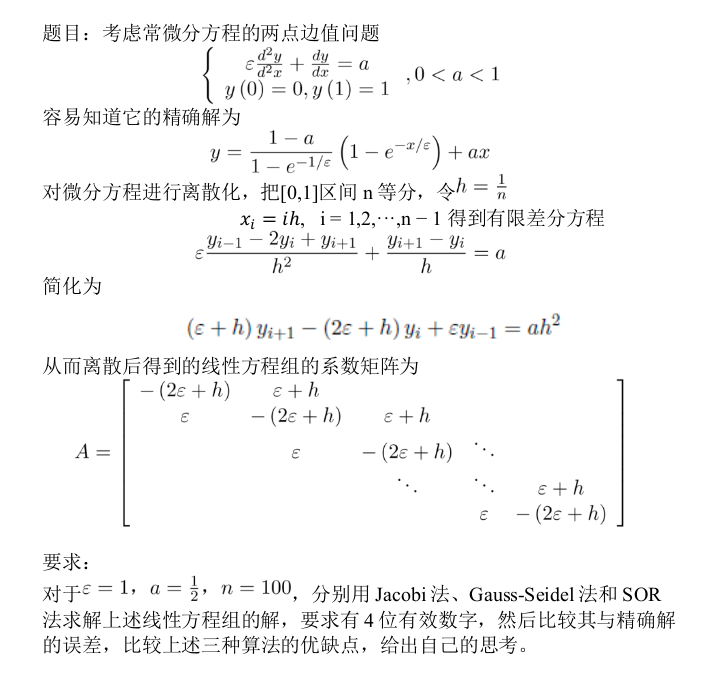
\includegraphics[width=5.5in]{problem.png}
        \caption{实验要求}
        \label{problem}
    \end{figure}
    
    \section{算法描述}
    \textbf{1.} Jacobi方法可以描述成为如下算法:
    \begin{algorithm}[!h]
        \centering
        \begin{algorithmic}[1]
            \Require $A,b$
            \Ensure $x$ such that $Ax = b$.
            \Procedure{Jacobi}{$A,b$}
                \State $x^{(0)} = (x_1^{(0)},\dots,x_n^{(0)})^T$.
                \For{$k=1,\dots,n$}
                    \State $x_i^{(k+1)} = (b_i - \sum_{j=1,j\neq i}^na_{ij}x_j^{(k)})/a_{ii},\forall i$.
                \EndFor
            \EndProcedure
        \end{algorithmic}
        \caption{Jacobi method}
        \label{jacobi}
    \end{algorithm}
    
    \textbf{2.} GS方法可以描述成为如下算法:
    \begin{algorithm}[!h]
        \centering
        \begin{algorithmic}[1]
            \Require $A,b$
            \Ensure $x$ such that $Ax = b$.
            \Procedure{GS}{$A,b$}
                \State $x^{(0)} = (x_1^{(0)},\dots,x_n^{(0)})^T$.
                \For{$k=1,\dots,n$}
                    \State $x_i^{(k+1)} = (b_i - \sum_{j=1}^{i-1}a_{ij}x_j^{(k+1)} - \sum_{j=i}^na_{ij}x_j^{(k)})/a_{ii},\forall i$.
                \EndFor
            \EndProcedure
        \end{algorithmic}
        \caption{GS method}
        \label{gs}
    \end{algorithm}
    
    \textbf{3.} SOR方法可以描述成为如下算法:
    \begin{algorithm}[!h]
        \centering
        \begin{algorithmic}[1]
            \Require $A,b$
            \Ensure $x$ such that $Ax = b$.
            \Procedure{SOR}{$A,b$}
                \State $x^{(0)} = (x_1^{(0)},\dots,x_n^{(0)})^T$.
                \For{$k=1,\dots,n$}
                    \State $x_i^{(k+1)} = x_i^{(k)} + \omega(b_i - \sum_{j=1}^{i-1}a_{ij}x_j^{(k+1)} - \sum_{j=i}^na_{ij}x_j^{(k)})/a_{ii},\forall i$.
                \EndFor
            \EndProcedure
        \end{algorithmic}
        \caption{SOR method}
        \label{sor}
    \end{algorithm}
        
    \section{程序清单}
    详细程序清单见表\ref{list}。
    \begin{table}[!htbp]
        \centering
        \begin{tabular}{c|c}
            \hline
            \hline
            文件名称 & 作用 \\
            \hline
            codes.cc & 实验代码\\
            iter.out & 实验结果输出文件\\
            report.tex & 实验报告源码\\
            report.pdf & 实验报告\\
            \hline
            \hline
        \end{tabular}
        \caption{程序清单}
        \label{list}
    \end{table}
    
    \section{运行结果}
    首先给出三种不同的迭代解方程的方法最终的迭代次数与产生的误差,见表\ref{res}。最终解得的向量在iter.out中给出。
    \begin{table}
        \centering
        \begin{tabular}{|l|l|l|}
        \hline\hline
        Method     & iteration & error     \\ \hline
        Jacobi     & 17724     & 0.00039   \\
        GS         & 8850      & 0.00040   \\
        SOR        & 3327      & 0.00033   \\ \hline
        \end{tabular}
        \caption{不同的矩阵迭代算法的迭代次数以及误差}
        \label{res}
    \end{table}

    在代码中,我们设$\epsilon = 1e-7$,当两次迭代之间所得向量的无穷范数小于$\epsilon$时,我们停止迭代。同时,我们选取SOR算法中的松弛参数为$1.5$。从结果中可以看出,从收敛的速度上来说,Jacobi方法最慢,GS其次,而SOR方法收敛速度最快。
    
    原始及完整运行结果在`iter.out'文件中给出。
        
    \section{体会与展望}
    通过这次迭代法解方程组的实验,更加深入地了解了迭代法解方程组的原理以及实现,更好的巩固了上课所学到的知识。
    
\end{document}